\PassOptionsToPackage{unicode=true}{hyperref} % options for packages loaded elsewhere
\PassOptionsToPackage{hyphens}{url}
%
\documentclass[]{article}
\usepackage{lmodern}
\usepackage{amssymb,amsmath}
\usepackage{ifxetex,ifluatex}
\usepackage{fixltx2e} % provides \textsubscript
\ifnum 0\ifxetex 1\fi\ifluatex 1\fi=0 % if pdftex
  \usepackage[T1]{fontenc}
  \usepackage[utf8]{inputenc}
  \usepackage{textcomp} % provides euro and other symbols
\else % if luatex or xelatex
  \usepackage{unicode-math}
  \defaultfontfeatures{Ligatures=TeX,Scale=MatchLowercase}
\fi
% use upquote if available, for straight quotes in verbatim environments
\IfFileExists{upquote.sty}{\usepackage{upquote}}{}
% use microtype if available
\IfFileExists{microtype.sty}{%
\usepackage[]{microtype}
\UseMicrotypeSet[protrusion]{basicmath} % disable protrusion for tt fonts
}{}
\IfFileExists{parskip.sty}{%
\usepackage{parskip}
}{% else
\setlength{\parindent}{0pt}
\setlength{\parskip}{6pt plus 2pt minus 1pt}
}
\usepackage{hyperref}
\hypersetup{
            pdfborder={0 0 0},
            breaklinks=true}
\urlstyle{same}  % don't use monospace font for urls
\usepackage[margin=1in]{geometry}
\usepackage{graphicx,grffile}
\makeatletter
\def\maxwidth{\ifdim\Gin@nat@width>\linewidth\linewidth\else\Gin@nat@width\fi}
\def\maxheight{\ifdim\Gin@nat@height>\textheight\textheight\else\Gin@nat@height\fi}
\makeatother
% Scale images if necessary, so that they will not overflow the page
% margins by default, and it is still possible to overwrite the defaults
% using explicit options in \includegraphics[width, height, ...]{}
\setkeys{Gin}{width=\maxwidth,height=\maxheight,keepaspectratio}
\setlength{\emergencystretch}{3em}  % prevent overfull lines
\providecommand{\tightlist}{%
  \setlength{\itemsep}{0pt}\setlength{\parskip}{0pt}}
\setcounter{secnumdepth}{0}
% Redefines (sub)paragraphs to behave more like sections
\ifx\paragraph\undefined\else
\let\oldparagraph\paragraph
\renewcommand{\paragraph}[1]{\oldparagraph{#1}\mbox{}}
\fi
\ifx\subparagraph\undefined\else
\let\oldsubparagraph\subparagraph
\renewcommand{\subparagraph}[1]{\oldsubparagraph{#1}\mbox{}}
\fi

% set default figure placement to htbp
\makeatletter
\def\fps@figure{htbp}
\makeatother


\author{}
\date{\vspace{-2.5em}}

\begin{document}

\hypertarget{conclusion}{%
\section{Conclusion}\label{conclusion}}

\hypertarget{political-party-affililation}{%
\subsubsection{Political Party
Affililation}\label{political-party-affililation}}

One of the interesting insight we gained from the dataset is the
distribution of the parties. Before gathering the data, we believe
Donald Trump will be the first among all other politicans. However, it
turns out that he was only the tenth place in total political ads
collected on Facebook. Ironically, while non-profit organization
occupied almost half of the top 20 ads, the frequency of Republican
ads(4.5\% of the top 20) were all focused on Donald Trump, pales in
comparsion to the 39.9\% apperance rate of Democrat ads. This data is
collected before

\includegraphics{Conclusion_files/figure-latex/unnamed-chunk-1-1.pdf}

\hypertarget{who-dominates-the-total-political-ads-collected}{%
\subsubsection{Who dominates the total political ads
collected}\label{who-dominates-the-total-political-ads-collected}}

Interestingly, the leader of the ads spent on Facebook are not from the
two parties. International Rescue Committee ends up the first in count /
frequency of ads collected. The following bar chart shows us how many
more ads are paid for by the Internaional Resuce Committee compared to
the 9 other organizations / partieswhich lag far behindl. While the
difference in ad count between the 2nd and 9th is close to 50, while
International Rescue Committee has a frequency of 255 ads collected.
This suggests that the ads from this ``non-profit organization'' exceeds
the other political campaign ads for candidates. However, the dataset
doesn't describe how much money is spent on each ads it's hard to
conclude that Internation Resuce Committee Spent the most money. For
example, an ads price can varies from the region, time, and all other
factors. Thus, we can only conclude that International Rescue committee
may spent the most effort on advertising, but not neccessary the most in
money spent.

\begin{figure}
\centering
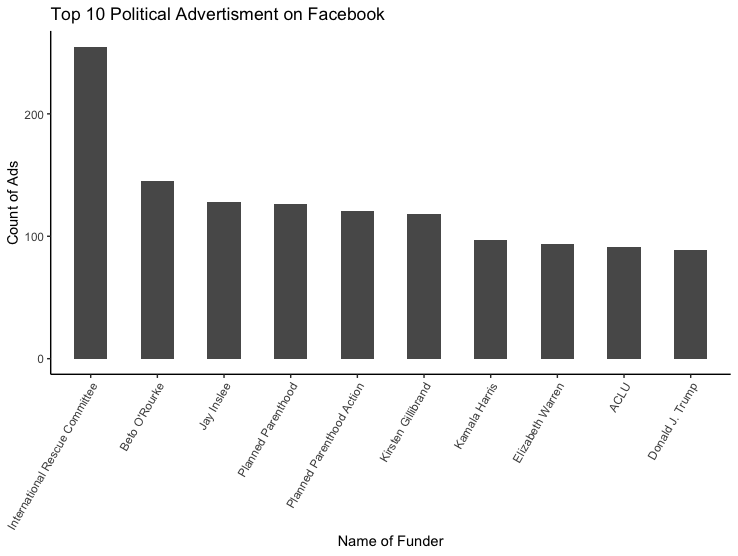
\includegraphics{data/Top10.png}
\caption{Top 10 Political Advertisment on Facebook}
\end{figure}

\end{document}
